\documentclass[]{article}
\usepackage{lmodern}
\usepackage{amssymb,amsmath}
\usepackage{ifxetex,ifluatex}
\usepackage{fixltx2e} % provides \textsubscript
\ifnum 0\ifxetex 1\fi\ifluatex 1\fi=0 % if pdftex
  \usepackage[T1]{fontenc}
  \usepackage[utf8]{inputenc}
\else % if luatex or xelatex
  \ifxetex
    \usepackage{mathspec}
  \else
    \usepackage{fontspec}
  \fi
  \defaultfontfeatures{Ligatures=TeX,Scale=MatchLowercase}
\fi
% use upquote if available, for straight quotes in verbatim environments
\IfFileExists{upquote.sty}{\usepackage{upquote}}{}
% use microtype if available
\IfFileExists{microtype.sty}{%
\usepackage{microtype}
\UseMicrotypeSet[protrusion]{basicmath} % disable protrusion for tt fonts
}{}
\usepackage[margin=1in]{geometry}
\usepackage{hyperref}
\hypersetup{unicode=true,
            pdfborder={0 0 0},
            breaklinks=true}
\urlstyle{same}  % don't use monospace font for urls
\usepackage{color}
\usepackage{fancyvrb}
\newcommand{\VerbBar}{|}
\newcommand{\VERB}{\Verb[commandchars=\\\{\}]}
\DefineVerbatimEnvironment{Highlighting}{Verbatim}{commandchars=\\\{\}}
% Add ',fontsize=\small' for more characters per line
\usepackage{framed}
\definecolor{shadecolor}{RGB}{248,248,248}
\newenvironment{Shaded}{\begin{snugshade}}{\end{snugshade}}
\newcommand{\KeywordTok}[1]{\textcolor[rgb]{0.13,0.29,0.53}{\textbf{#1}}}
\newcommand{\DataTypeTok}[1]{\textcolor[rgb]{0.13,0.29,0.53}{#1}}
\newcommand{\DecValTok}[1]{\textcolor[rgb]{0.00,0.00,0.81}{#1}}
\newcommand{\BaseNTok}[1]{\textcolor[rgb]{0.00,0.00,0.81}{#1}}
\newcommand{\FloatTok}[1]{\textcolor[rgb]{0.00,0.00,0.81}{#1}}
\newcommand{\ConstantTok}[1]{\textcolor[rgb]{0.00,0.00,0.00}{#1}}
\newcommand{\CharTok}[1]{\textcolor[rgb]{0.31,0.60,0.02}{#1}}
\newcommand{\SpecialCharTok}[1]{\textcolor[rgb]{0.00,0.00,0.00}{#1}}
\newcommand{\StringTok}[1]{\textcolor[rgb]{0.31,0.60,0.02}{#1}}
\newcommand{\VerbatimStringTok}[1]{\textcolor[rgb]{0.31,0.60,0.02}{#1}}
\newcommand{\SpecialStringTok}[1]{\textcolor[rgb]{0.31,0.60,0.02}{#1}}
\newcommand{\ImportTok}[1]{#1}
\newcommand{\CommentTok}[1]{\textcolor[rgb]{0.56,0.35,0.01}{\textit{#1}}}
\newcommand{\DocumentationTok}[1]{\textcolor[rgb]{0.56,0.35,0.01}{\textbf{\textit{#1}}}}
\newcommand{\AnnotationTok}[1]{\textcolor[rgb]{0.56,0.35,0.01}{\textbf{\textit{#1}}}}
\newcommand{\CommentVarTok}[1]{\textcolor[rgb]{0.56,0.35,0.01}{\textbf{\textit{#1}}}}
\newcommand{\OtherTok}[1]{\textcolor[rgb]{0.56,0.35,0.01}{#1}}
\newcommand{\FunctionTok}[1]{\textcolor[rgb]{0.00,0.00,0.00}{#1}}
\newcommand{\VariableTok}[1]{\textcolor[rgb]{0.00,0.00,0.00}{#1}}
\newcommand{\ControlFlowTok}[1]{\textcolor[rgb]{0.13,0.29,0.53}{\textbf{#1}}}
\newcommand{\OperatorTok}[1]{\textcolor[rgb]{0.81,0.36,0.00}{\textbf{#1}}}
\newcommand{\BuiltInTok}[1]{#1}
\newcommand{\ExtensionTok}[1]{#1}
\newcommand{\PreprocessorTok}[1]{\textcolor[rgb]{0.56,0.35,0.01}{\textit{#1}}}
\newcommand{\AttributeTok}[1]{\textcolor[rgb]{0.77,0.63,0.00}{#1}}
\newcommand{\RegionMarkerTok}[1]{#1}
\newcommand{\InformationTok}[1]{\textcolor[rgb]{0.56,0.35,0.01}{\textbf{\textit{#1}}}}
\newcommand{\WarningTok}[1]{\textcolor[rgb]{0.56,0.35,0.01}{\textbf{\textit{#1}}}}
\newcommand{\AlertTok}[1]{\textcolor[rgb]{0.94,0.16,0.16}{#1}}
\newcommand{\ErrorTok}[1]{\textcolor[rgb]{0.64,0.00,0.00}{\textbf{#1}}}
\newcommand{\NormalTok}[1]{#1}
\usepackage{graphicx,grffile}
\makeatletter
\def\maxwidth{\ifdim\Gin@nat@width>\linewidth\linewidth\else\Gin@nat@width\fi}
\def\maxheight{\ifdim\Gin@nat@height>\textheight\textheight\else\Gin@nat@height\fi}
\makeatother
% Scale images if necessary, so that they will not overflow the page
% margins by default, and it is still possible to overwrite the defaults
% using explicit options in \includegraphics[width, height, ...]{}
\setkeys{Gin}{width=\maxwidth,height=\maxheight,keepaspectratio}
\IfFileExists{parskip.sty}{%
\usepackage{parskip}
}{% else
\setlength{\parindent}{0pt}
\setlength{\parskip}{6pt plus 2pt minus 1pt}
}
\setlength{\emergencystretch}{3em}  % prevent overfull lines
\providecommand{\tightlist}{%
  \setlength{\itemsep}{0pt}\setlength{\parskip}{0pt}}
\setcounter{secnumdepth}{0}
% Redefines (sub)paragraphs to behave more like sections
\ifx\paragraph\undefined\else
\let\oldparagraph\paragraph
\renewcommand{\paragraph}[1]{\oldparagraph{#1}\mbox{}}
\fi
\ifx\subparagraph\undefined\else
\let\oldsubparagraph\subparagraph
\renewcommand{\subparagraph}[1]{\oldsubparagraph{#1}\mbox{}}
\fi

%%% Use protect on footnotes to avoid problems with footnotes in titles
\let\rmarkdownfootnote\footnote%
\def\footnote{\protect\rmarkdownfootnote}

%%% Change title format to be more compact
\usepackage{titling}

% Create subtitle command for use in maketitle
\newcommand{\subtitle}[1]{
  \posttitle{
    \begin{center}\large#1\end{center}
    }
}

\setlength{\droptitle}{-2em}

  \title{\begin{enumerate}
\def\labelenumi{\arabic{enumi}.}
\setcounter{enumi}{2}
\tightlist
\item
  Visualisasi Data Menggunakan Fungsi Dasar R
\end{enumerate}}
    \pretitle{\vspace{\droptitle}\centering\huge}
  \posttitle{\par}
    \author{}
    \preauthor{}\postauthor{}
      \predate{\centering\large\emph}
  \postdate{\par}
    \date{2019-03-09T00:00:00+07:00}


\begin{document}
\maketitle

\begin{quote}
\textbf{Note: }

\begin{itemize}
\tightlist
\item
  \href{Visualisasi\%20Data\%20Menggunakan\%20Fungsi\%20plot}{}{[}\#4-1-visualisasi-data-menggunakan-fungsi-plot{]}
\end{itemize}
\end{quote}

\subsection{4.1 Visualisasi Data Menggunakan Fungsi
plot()}\label{visualisasi-data-menggunakan-fungsi-plot}

Fungsi \texttt{plot()} merupakan fungsi umum yang digunakan untuk
membuat plot pada \texttt{R}. Format dasarnya adalah sebagai berikut:

\begin{Shaded}
\begin{Highlighting}[]
\KeywordTok{plot}\NormalTok{(x, y, }\DataTypeTok{type=}\StringTok{"p"}\NormalTok{)}
\end{Highlighting}
\end{Shaded}

\begin{quote}
\textbf{Note: }

\begin{itemize}
\tightlist
\item
  \textbf{x dan y}: titik koordinat plot Berupa variabel dengan panjang
  atau jumlah observasi yang sama.
\item
  \textbf{type}: jenis grafik yang hendak dibuat. Nilai yang dapat
  dimasukkan antara lain:
\item
  type=``p'' : membuat plot titik atau scatterplot. Nilai ini merupakan
  default pada fungsi \texttt{plot()}.
\item
  type=``l'' : membuat plot garis.
\item
  type=``b'' : membuat plot titik yang terhubung dengan garis.
\item
  type=``o'' : membuat plot titik yang ditimpa oleh garis.
\item
  type=``h'' : membuat plot garis vertikal dari titik ke garis y=0.
\item
  type=``s'' : membuat fungsi tangga.
\item
  type=``n'' : tidak membuat grafik plot sama sekali, kecuali plot dari
  axis. Dapat digunakan untuk mengatur tampilan suatu plot utama yang
  diikuti oleh sekelompok plot tambahan.
\end{itemize}
\end{quote}

Untuk lebih memahaminya berikut penulis akan sajikan contoh untuk
masing-masing grafik tersebut. Berikut adalah contoh sintaks dan hasil
plot yang disajikan pada Figure @ref(fig:plot):

\begin{Shaded}
\begin{Highlighting}[]
\CommentTok{# membuat vektor data }
\NormalTok{x <-}\StringTok{ }\KeywordTok{c}\NormalTok{(}\DecValTok{1}\OperatorTok{:}\DecValTok{10}\NormalTok{); y <-}\StringTok{ }\NormalTok{x}\OperatorTok{^}\DecValTok{2}
\end{Highlighting}
\end{Shaded}

\begin{Shaded}
\begin{Highlighting}[]
\KeywordTok{plot}\NormalTok{(x, y, }\DataTypeTok{type=}\StringTok{"p"}\NormalTok{)}
\end{Highlighting}
\end{Shaded}

\begin{figure}

{\centering 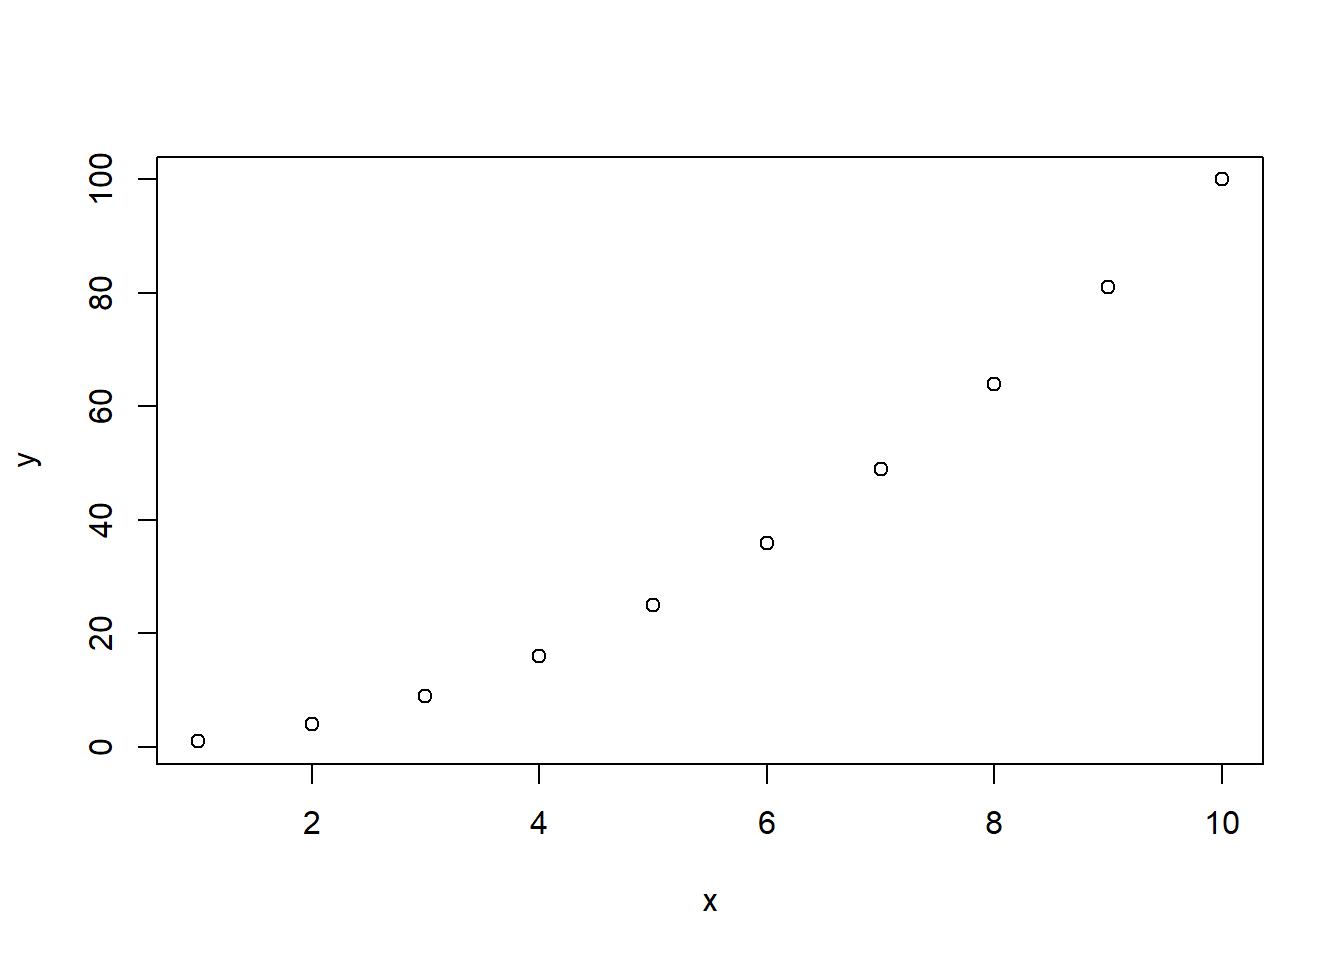
\includegraphics{04_visualisasi-data-menggunakan-fungsi-dasar-r_files/figure-latex/plot-1} 

}

\caption{Plot berbagai jenis setting type}\label{fig:plot1}
\end{figure}

\begin{Shaded}
\begin{Highlighting}[]
\KeywordTok{plot}\NormalTok{(x, y, }\DataTypeTok{type=}\StringTok{"l"}\NormalTok{)}
\end{Highlighting}
\end{Shaded}

\begin{figure}

{\centering 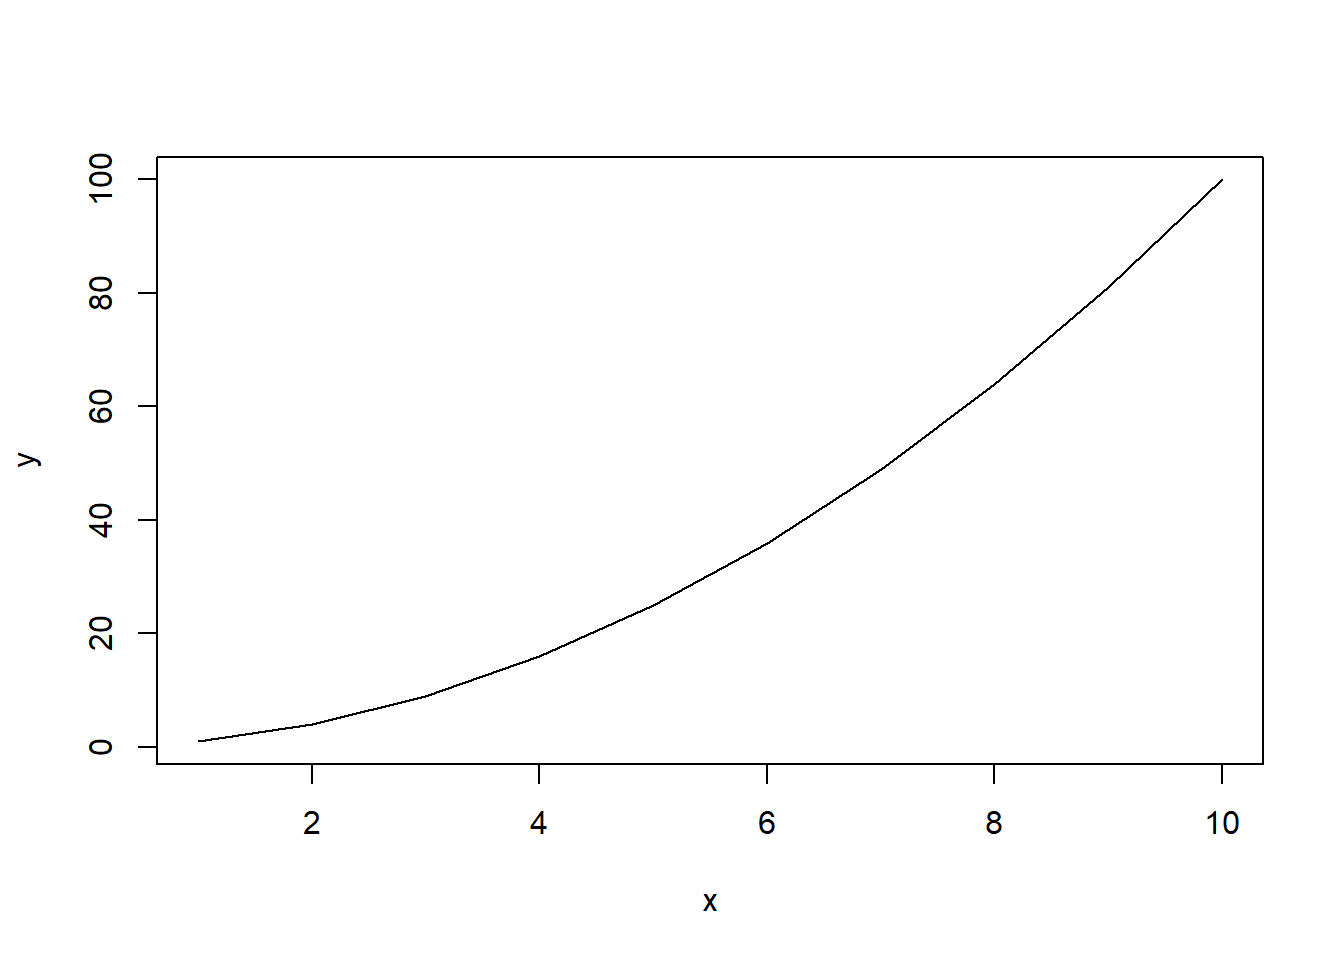
\includegraphics{04_visualisasi-data-menggunakan-fungsi-dasar-r_files/figure-latex/plot-2} 

}

\caption{Plot berbagai jenis setting type}\label{fig:plot2}
\end{figure}

\begin{Shaded}
\begin{Highlighting}[]
\KeywordTok{plot}\NormalTok{(x, y, }\DataTypeTok{type=}\StringTok{"b"}\NormalTok{)}
\end{Highlighting}
\end{Shaded}

\begin{figure}

{\centering 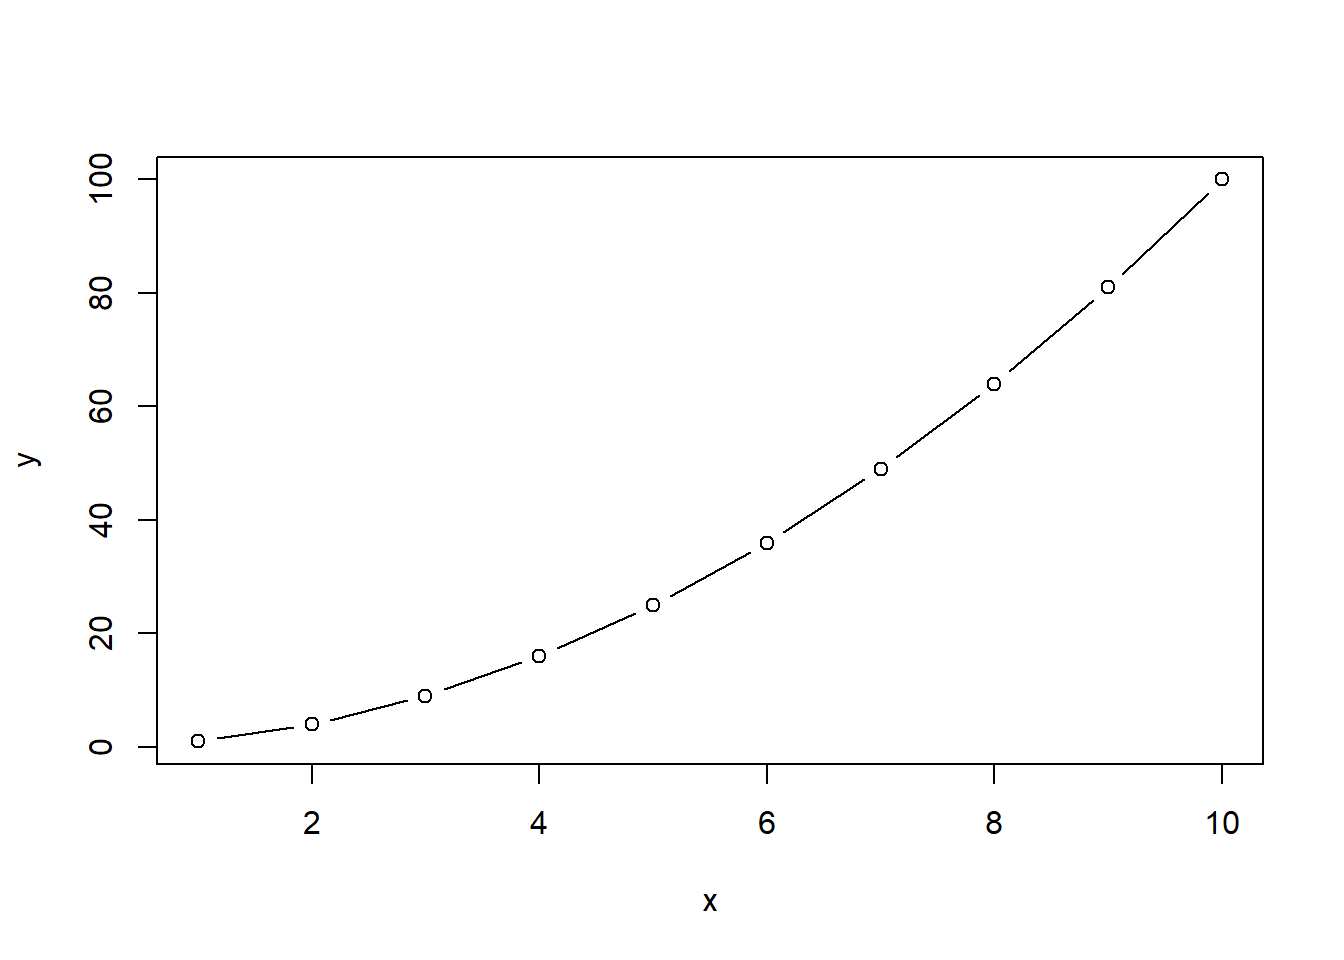
\includegraphics{04_visualisasi-data-menggunakan-fungsi-dasar-r_files/figure-latex/plot-3} 

}

\caption{Plot berbagai jenis setting type}\label{fig:plot3}
\end{figure}

\begin{Shaded}
\begin{Highlighting}[]
\KeywordTok{plot}\NormalTok{(x, y, }\DataTypeTok{type=}\StringTok{"o"}\NormalTok{)}
\end{Highlighting}
\end{Shaded}

\begin{figure}

{\centering 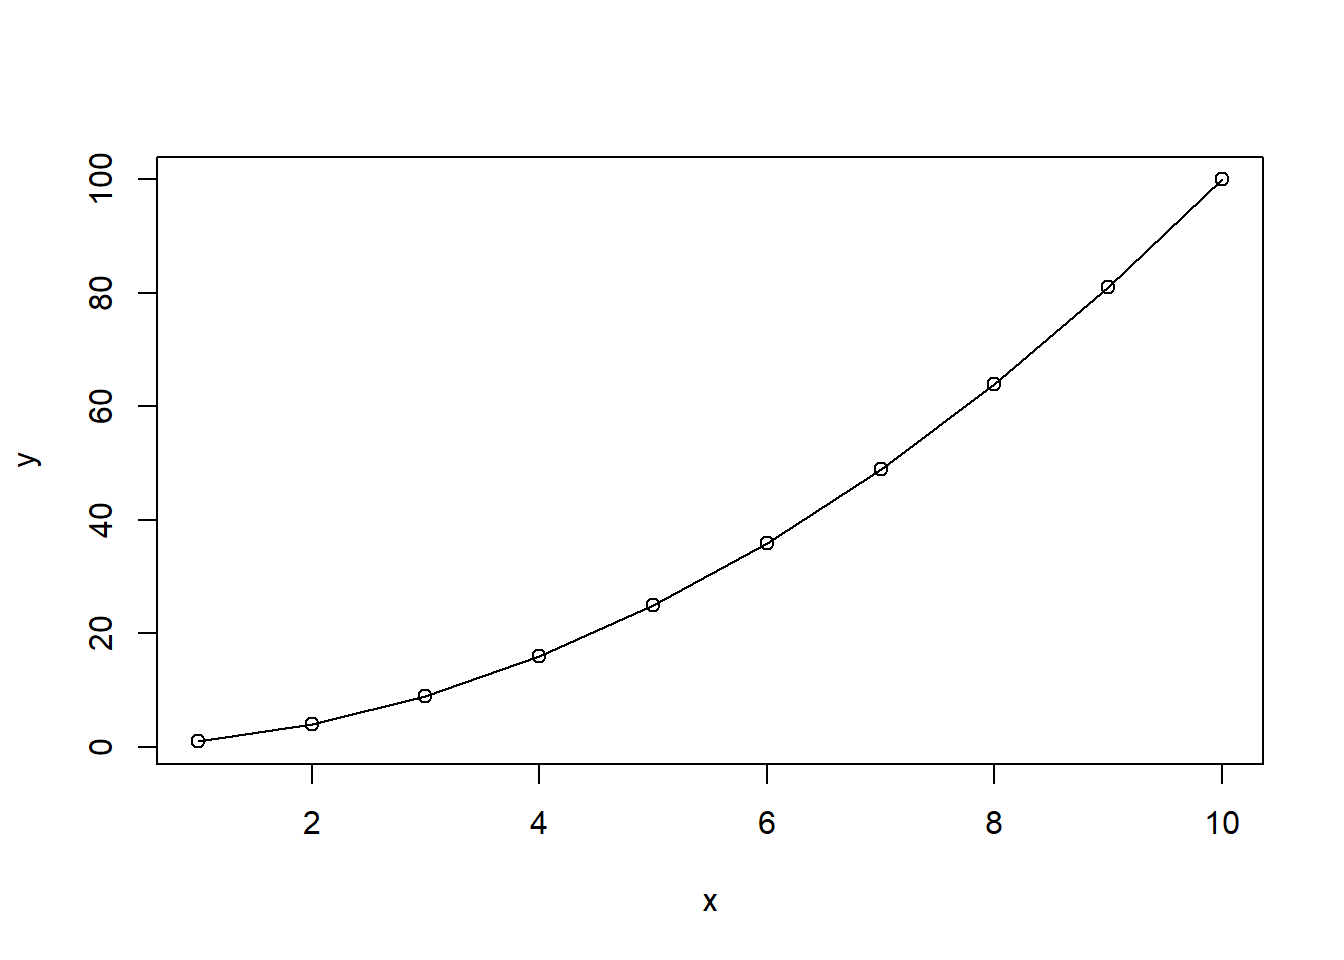
\includegraphics{04_visualisasi-data-menggunakan-fungsi-dasar-r_files/figure-latex/plot-4} 

}

\caption{Plot berbagai jenis setting type}\label{fig:plot4}
\end{figure}

\begin{Shaded}
\begin{Highlighting}[]
\KeywordTok{plot}\NormalTok{(x, y, }\DataTypeTok{type=}\StringTok{"h"}\NormalTok{)}
\end{Highlighting}
\end{Shaded}

\begin{figure}

{\centering 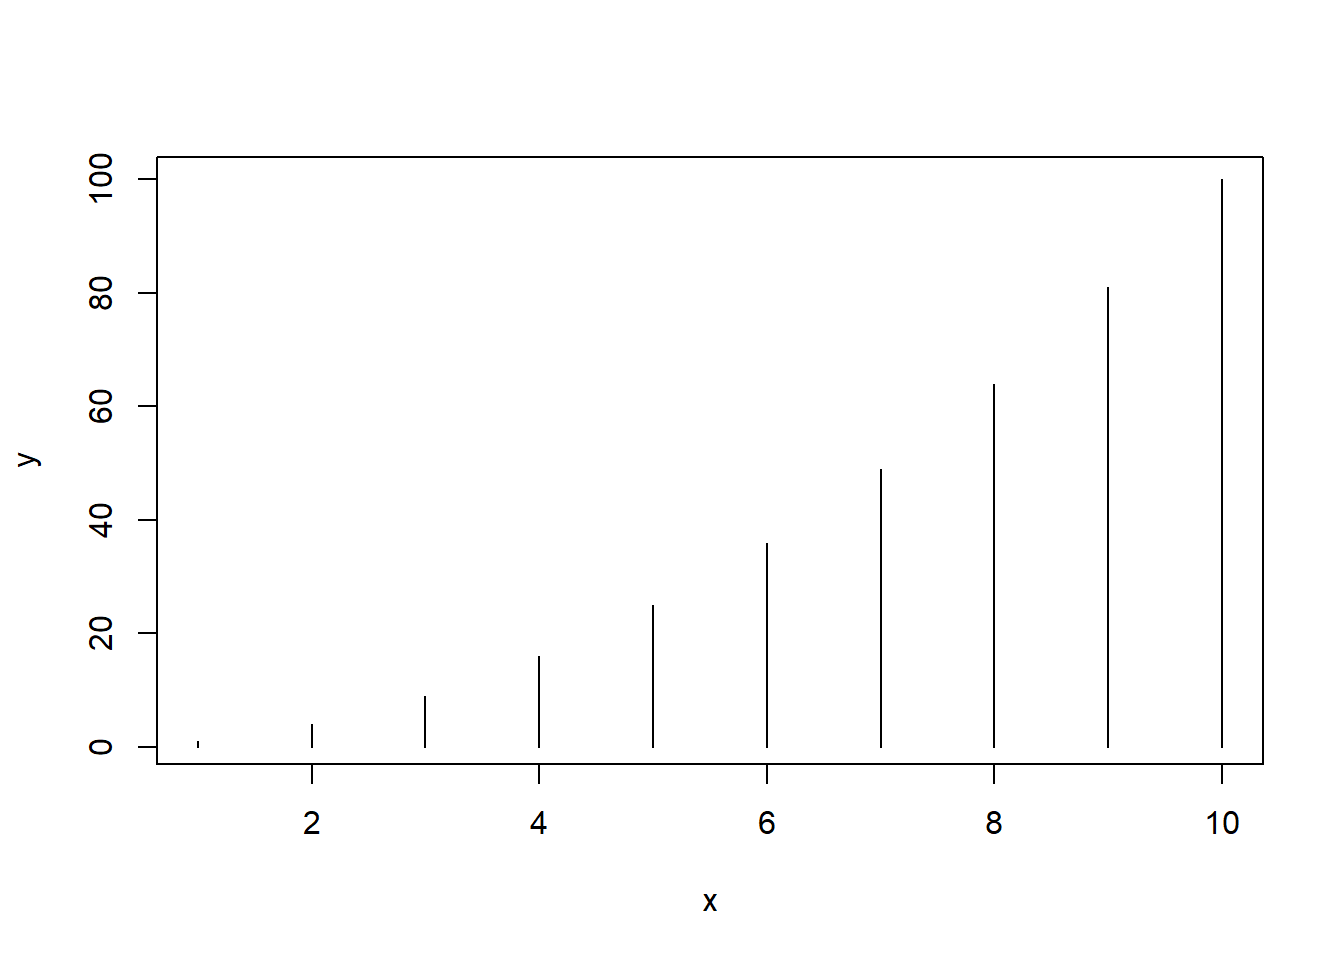
\includegraphics{04_visualisasi-data-menggunakan-fungsi-dasar-r_files/figure-latex/plot-5} 

}

\caption{Plot berbagai jenis setting type}\label{fig:plot5}
\end{figure}

\begin{Shaded}
\begin{Highlighting}[]
\KeywordTok{plot}\NormalTok{(x, y, }\DataTypeTok{type=}\StringTok{"s"}\NormalTok{)}
\end{Highlighting}
\end{Shaded}

\begin{figure}

{\centering 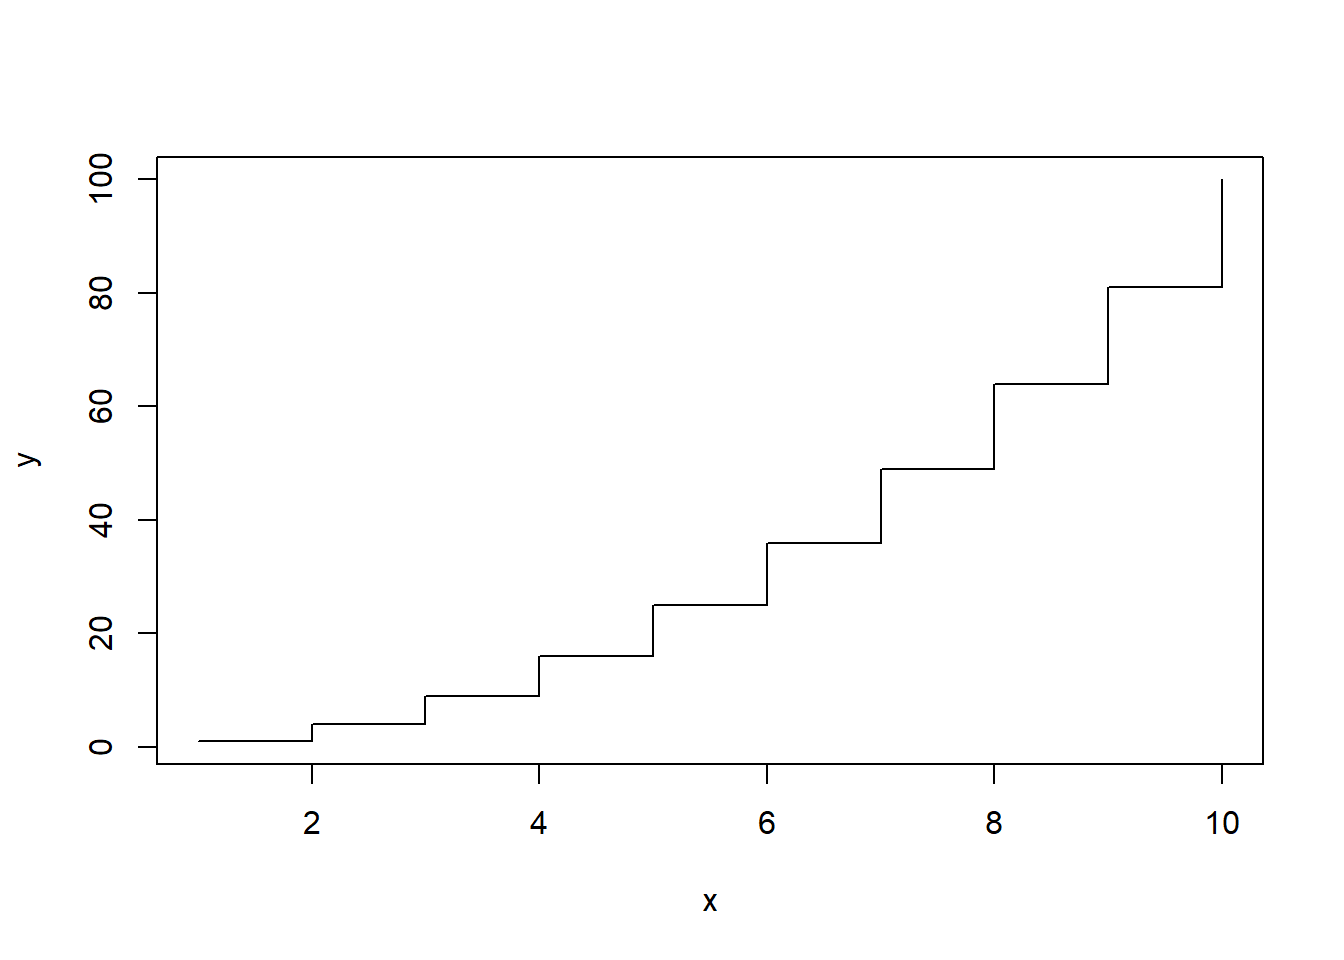
\includegraphics{04_visualisasi-data-menggunakan-fungsi-dasar-r_files/figure-latex/plot-6} 

}

\caption{Plot berbagai jenis setting type}\label{fig:plot6}
\end{figure}

\begin{Shaded}
\begin{Highlighting}[]
\KeywordTok{plot}\NormalTok{(x, y, }\DataTypeTok{type=}\StringTok{"n"}\NormalTok{)}
\end{Highlighting}
\end{Shaded}

\begin{figure}

{\centering 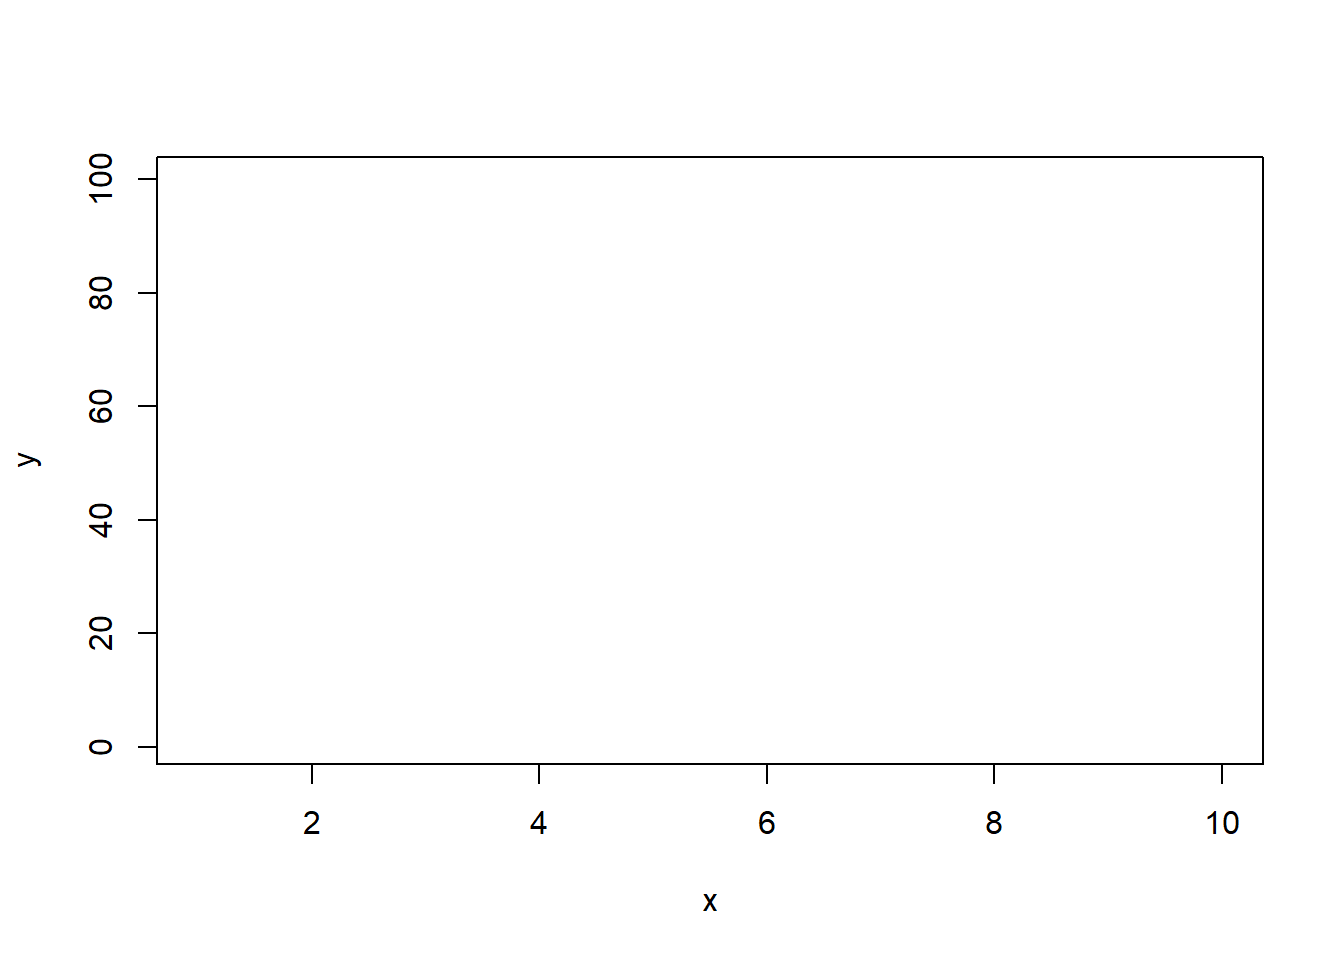
\includegraphics{04_visualisasi-data-menggunakan-fungsi-dasar-r_files/figure-latex/plot-7} 

}

\caption{Plot berbagai jenis setting type}\label{fig:plot7}
\end{figure}

Pada contoh selanjutnya akan dilakukan plot terhadap dataset
\texttt{trees}. Untuk memuatnya jalankan sintaks berikut:

\begin{Shaded}
\begin{Highlighting}[]
\KeywordTok{library}\NormalTok{(tibble)}
\end{Highlighting}
\end{Shaded}

\begin{Shaded}
\begin{Highlighting}[]
\CommentTok{# memuat dataset}
\NormalTok{trees <-}\StringTok{ }\KeywordTok{as_tibble}\NormalTok{(trees)}

\CommentTok{# print }
\NormalTok{trees}
\end{Highlighting}
\end{Shaded}

\begin{verbatim}
## # A tibble: 31 x 3
##    Girth Height Volume
##    <dbl>  <dbl>  <dbl>
##  1   8.3     70   10.3
##  2   8.6     65   10.3
##  3   8.8     63   10.2
##  4  10.5     72   16.4
##  5  10.7     81   18.8
##  6  10.8     83   19.7
##  7  11       66   15.6
##  8  11       75   18.2
##  9  11.1     80   22.6
## 10  11.2     75   19.9
## # ... with 21 more rows
\end{verbatim}

Pada dataset tersebut kita ingin membuat scatterplot untuk melihat
korelasi antara variabel \texttt{Height} dan \texttt{Volume}. Untuk
melakukannya jalankan sintaks berikut:

\begin{Shaded}
\begin{Highlighting}[]
\KeywordTok{plot}\NormalTok{(trees}\OperatorTok{$}\NormalTok{Height, trees}\OperatorTok{$}\NormalTok{Volume)}
\end{Highlighting}
\end{Shaded}

\begin{Shaded}
\begin{Highlighting}[]
\CommentTok{# atau }
\KeywordTok{with}\NormalTok{(trees, }\KeywordTok{plot}\NormalTok{(Height, Volume))}
\end{Highlighting}
\end{Shaded}

\begin{figure}

{\centering 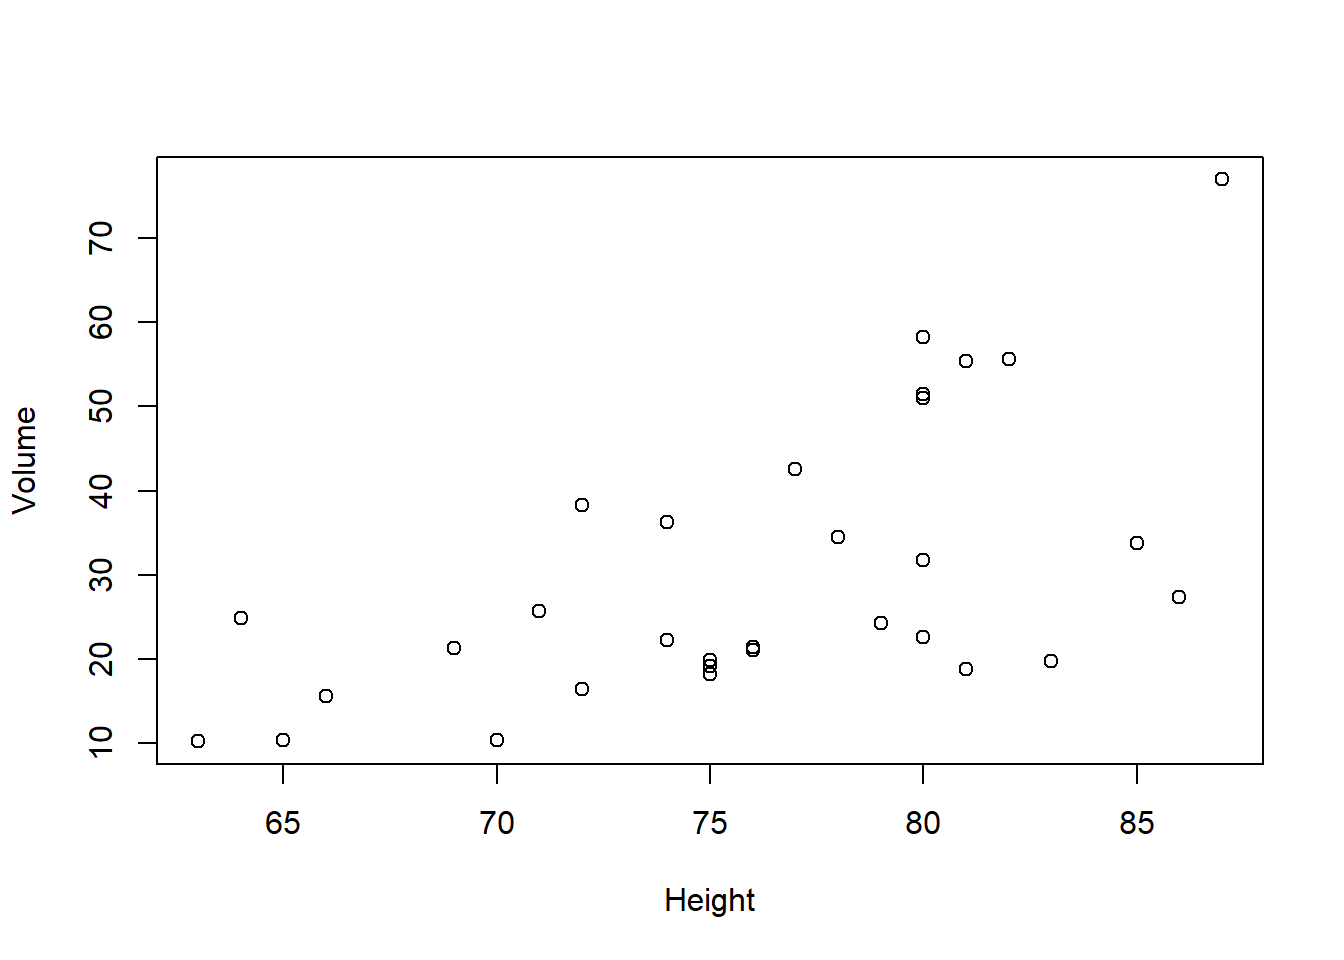
\includegraphics{04_visualisasi-data-menggunakan-fungsi-dasar-r_files/figure-latex/scatter-1} 

}

\caption{Scatterplot Height vs Volume}\label{fig:scatter}
\end{figure}

Kita juga dapat menggunakan formula untuk membuat scatterplot pada
Figure @ref(fig:scatter). Berikut adalah contoh sintaks yang digunakan:

\begin{Shaded}
\begin{Highlighting}[]
\NormalTok{x <-}\StringTok{ }\NormalTok{trees}\OperatorTok{$}\NormalTok{Height}
\NormalTok{y <-}\StringTok{ }\NormalTok{trees}\OperatorTok{$}\NormalTok{Volume}

\KeywordTok{plot}\NormalTok{(y}\OperatorTok{~}\NormalTok{x)}
\end{Highlighting}
\end{Shaded}

Fungsi \texttt{plot()} juga dapat digunakan untuk membentuk matriks
scatterplot. Untuk membuatnya kita hanya perlu memasukkan seluruh
dataset kedalam fungsi \texttt{plot()}. Berikut adalah contoh sintaks


\end{document}
